% ---------------------------
% Put these in your document preamble:
% ---------------------------
% \usepackage{graphicx}   % for \includegraphics
% \usepackage{float}      % for [H]
% \usepackage{placeins}   % for \FloatBarrier (keep floats from moving past a barrier)
% \usepackage{caption}    % if you need \captionof or extra caption control
% ---------------------------

% Appendix (body)
\chapter*{Appendix} % Main appendix title
\label{Appendix}


% ======================================================================
% ======================================================================
% 
%
%                                Development
%
%
% ======================================================================
% ======================================================================

\section*{Development Structure}
\label{appendix:dev-structure}
TODO --> Insert coding development structure here on how to utilize the package 
correctly (maybe a README)



% ======================================================================
% ======================================================================
% 
%
%                               Ranks Comparison
%
%
% ======================================================================
% ======================================================================
\section*{Token Ranks Comparison}



% ======================================================================
\subsection*{Model \textit{HuggingFaceTB/SmolLM2-135M}}

% ---------------------------------------------
\subsubsection*{Number New Tokens = 1000}
\begin{figure}[H]
    \centering
    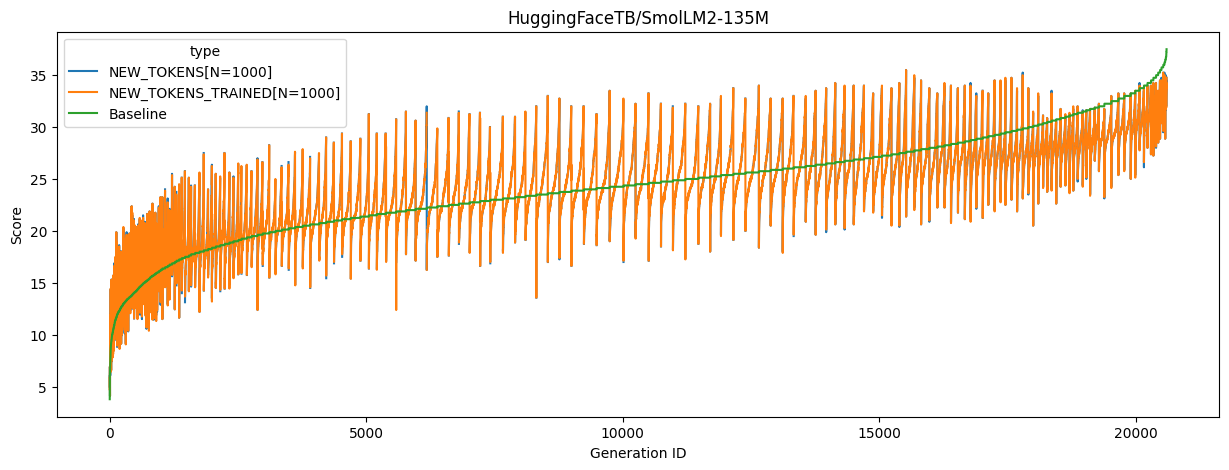
\includegraphics[width=\textwidth]{Figures/Appendix/token-rank-comparison_1000_smol135M.png}
    \caption{Score comparison between original sub-token sequences and newly introduced tokens. Higher ranks indicate higher model preference.}
    \label{fig:new_token_rank:1000_smol135M}
\end{figure}
\FloatBarrier
% ---------------------------------------------
\subsubsection*{Number New Tokens = 5000}
\begin{figure}[H]
    \centering
    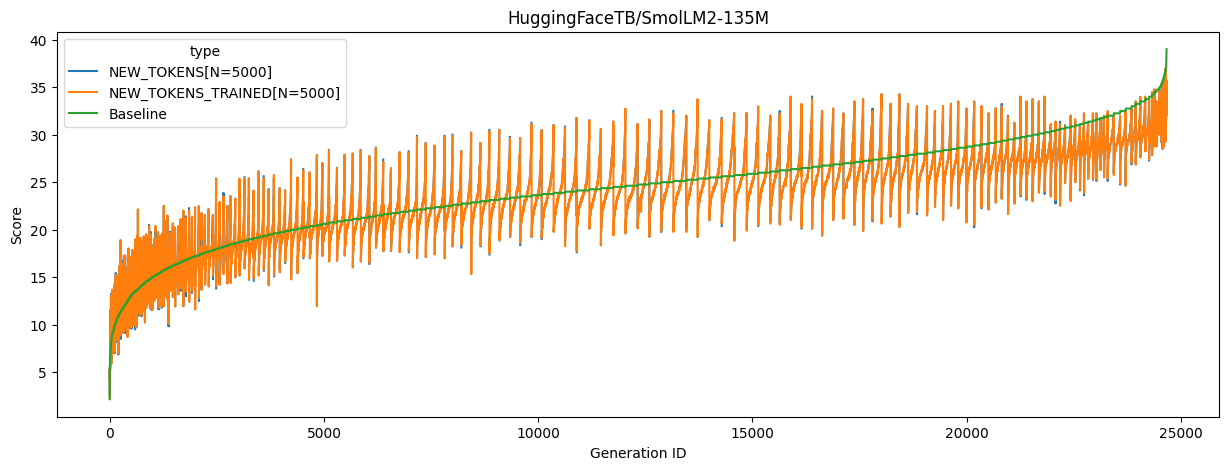
\includegraphics[width=\textwidth]{Figures/Appendix/token-rank-comparison_5000_smol135M.png}
    \caption{Score comparison between original sub-token sequences and newly introduced tokens. Higher ranks indicate higher model preference.}
    \label{fig:new_token_rank:5000_smol135M}
\end{figure}
\FloatBarrier
% ---------------------------------------------
\subsubsection*{Number New Tokens = 7500}
\begin{figure}[H]
    \centering
    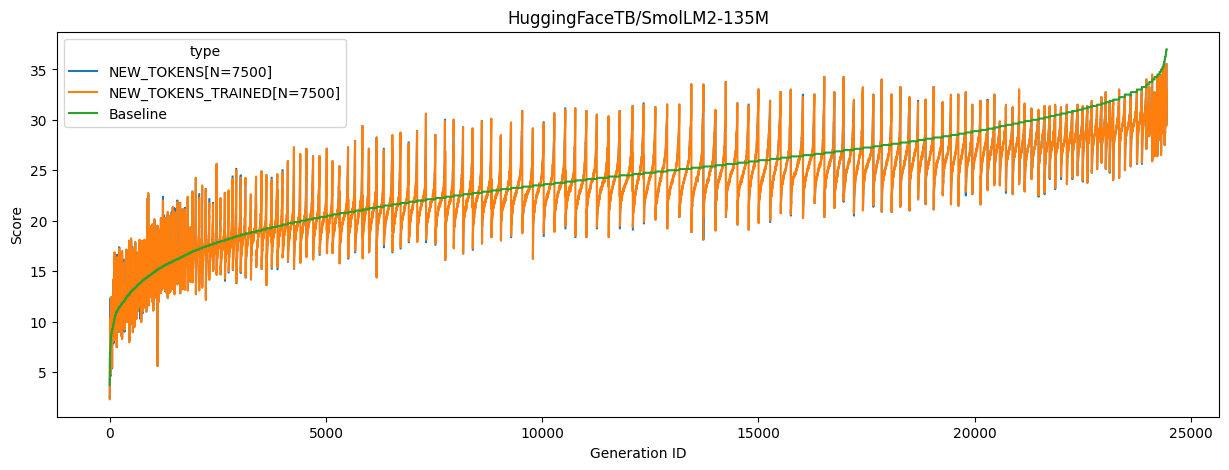
\includegraphics[width=\textwidth]{Figures/Appendix/token-rank-comparison_7500_smol135M.png}
    \caption{Score comparison between original sub-token sequences and newly introduced tokens. Higher ranks indicate higher model preference.}
    \label{fig:new_token_rank:7500_smol135M}
\end{figure}
\FloatBarrier
% ---------------------------------------------


% ======================================================================
\subsection*{Model \textit{Qwen/Qwen2.5-1.5B-Instruct}}

% ---------------------------------------------
\subsubsection*{Number New Tokens = 1000}
\begin{figure}[H]
    \centering
    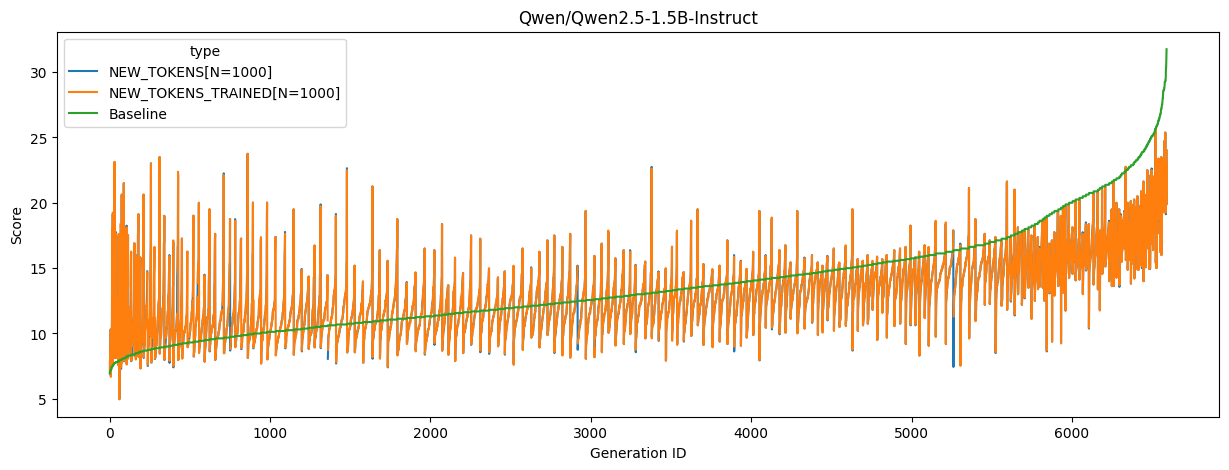
\includegraphics[width=\textwidth]{Figures/Appendix/token-rank-comparison_1000_qwen.png}
    \caption{Score comparison between original sub-token sequences and newly introduced tokens. Higher ranks indicate higher model preference.}
    \label{fig:new_token_rank:1000_qwen}
\end{figure}
\FloatBarrier
% ---------------------------------------------
\subsubsection*{Number New Tokens = 5000}
\begin{figure}[H]
    \centering
    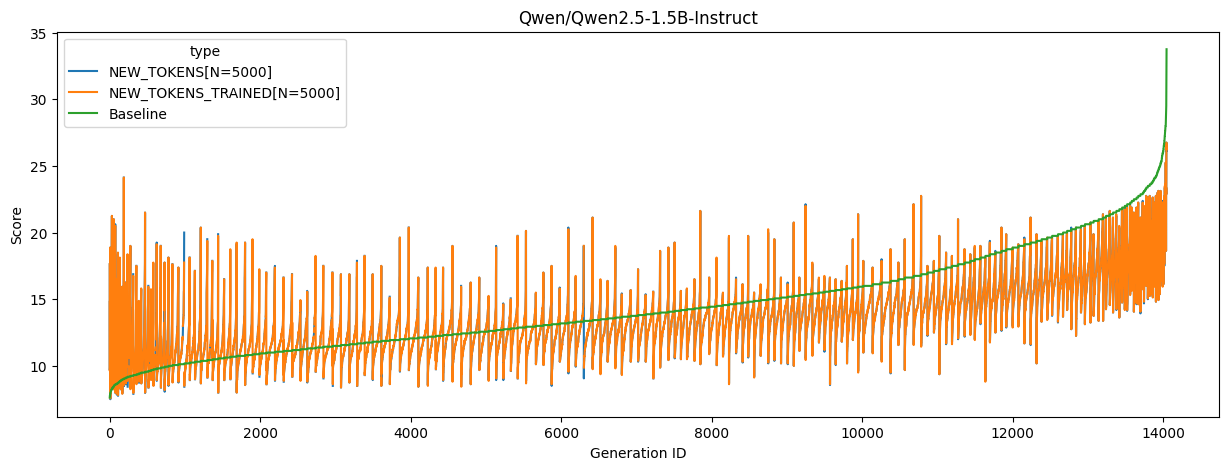
\includegraphics[width=\textwidth]{Figures/Appendix/token-rank-comparison_5000_qwen.png}
    \caption{Score comparison between original sub-token sequences and newly introduced tokens. Higher ranks indicate higher model preference.}
    \label{fig:new_token_rank:5000_qwen}
\end{figure}
\FloatBarrier
% ---------------------------------------------

\subsubsection*{Number New Tokens = 7500}
\begin{figure}[H]
    \centering
    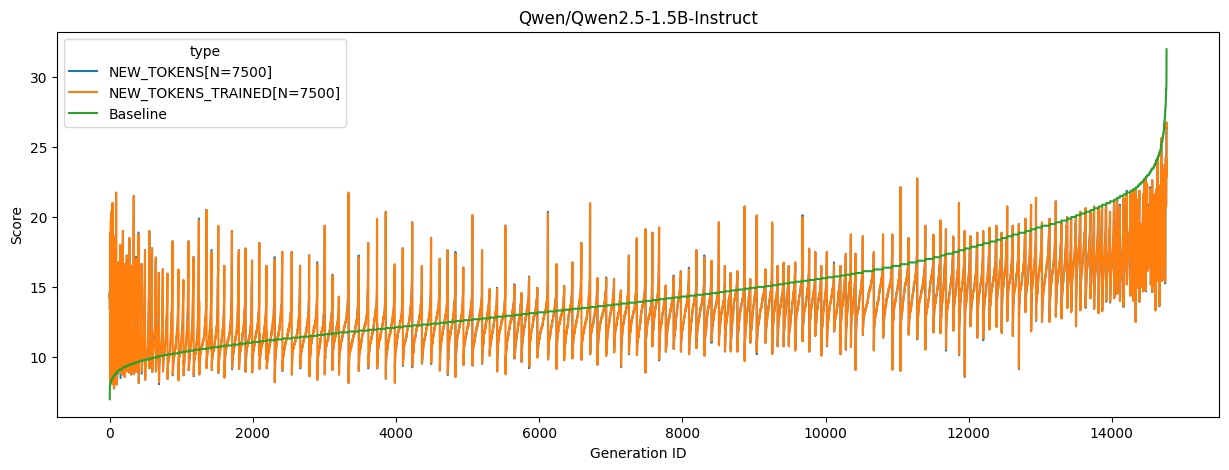
\includegraphics[width=\textwidth]{Figures/Appendix/token-rank-comparison_7500_qwen.png}
    \caption{Score comparison between original sub-token sequences and newly introduced tokens. Higher ranks indicate higher model preference.}
    \label{fig:new_token_rank:7500_qwen}
\end{figure}
\FloatBarrier
% ---------------------------------------------


% ======================================================================
\subsection*{Model \textit{HuggingFaceTB/SmolLM3-3B}}

% ---------------------------------------------
\subsubsection*{Number New Tokens = 1000}
\begin{figure}[H]
    \centering
    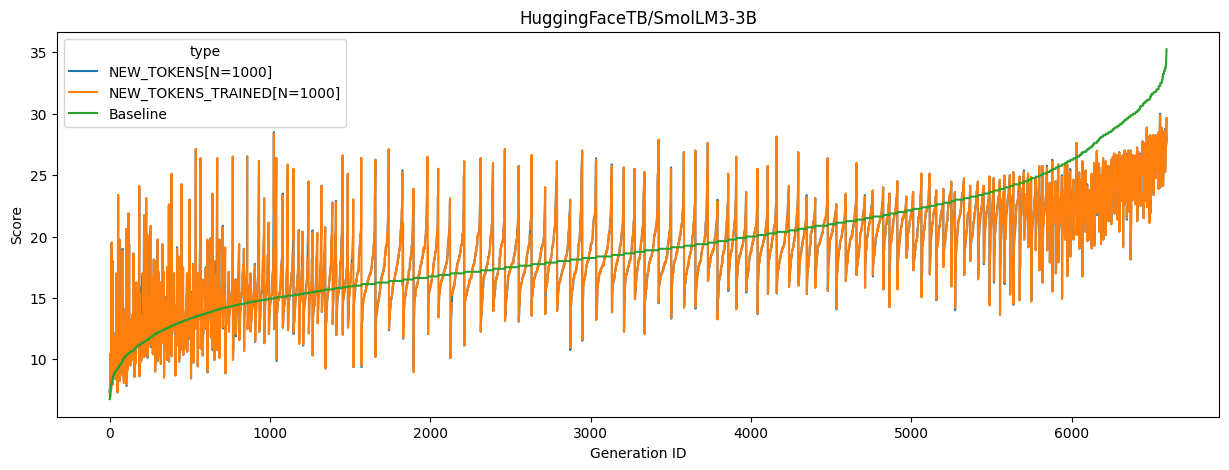
\includegraphics[width=\textwidth]{Figures/Appendix/token-rank-comparison_1000_smol3B.png}
    \caption{Score comparison between original sub-token sequences and newly introduced tokens. Higher ranks indicate higher model preference.}
    \label{fig:new_token_rank:1000_smol3B}
\end{figure}
\FloatBarrier
% ---------------------------------------------

\subsubsection*{Number New Tokens = 5000}
\begin{figure}[H]
    \centering
    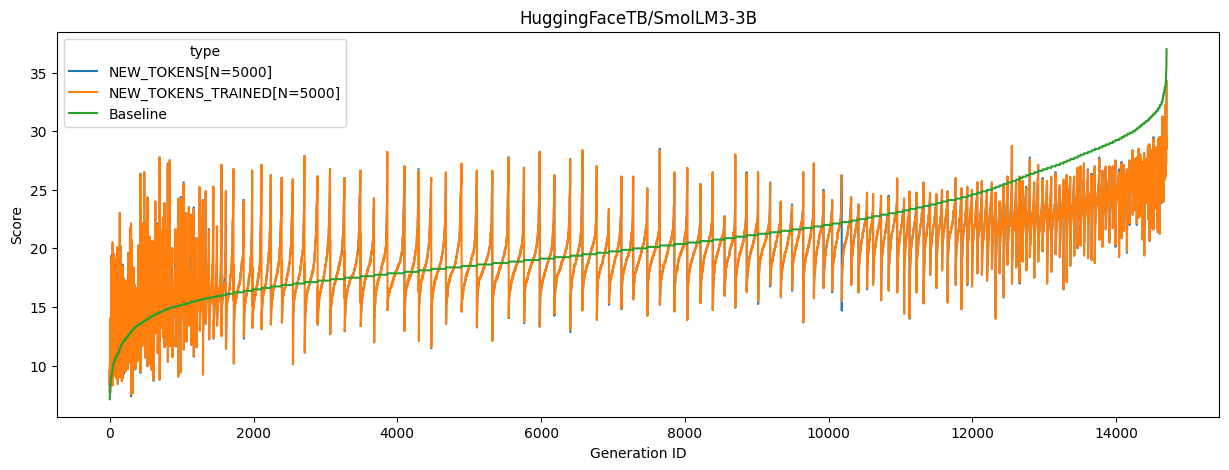
\includegraphics[width=\textwidth]{Figures/Appendix/token-rank-comparison_5000_smol3B.png}
    \caption{Score comparison between original sub-token sequences and newly introduced tokens. Higher ranks indicate higher model preference.}
    \label{fig:new_token_rank:5000_smol3B}
\end{figure}
\FloatBarrier
% ---------------------------------------------

\subsubsection*{Number New Tokens = 7500}
\begin{figure}[H]
    \centering
    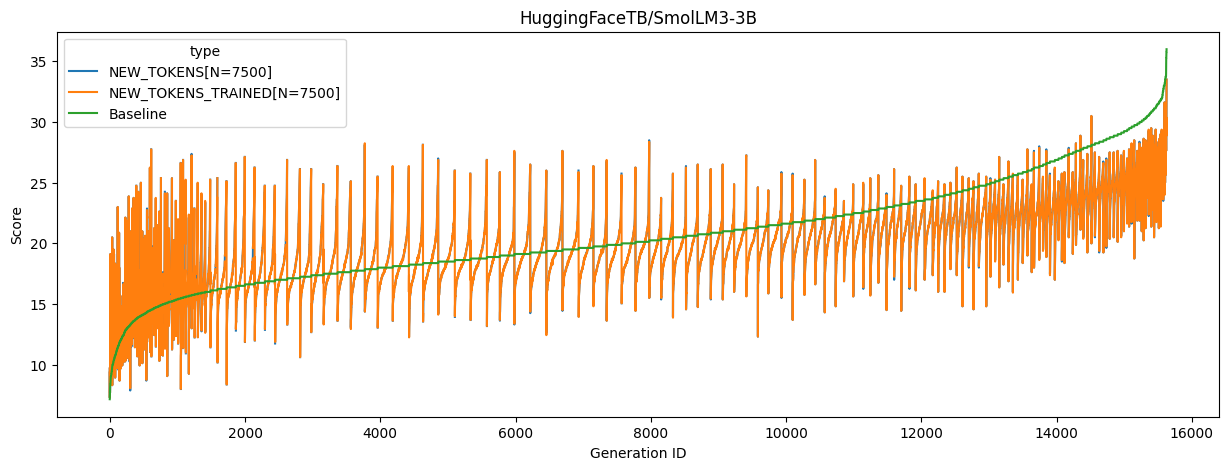
\includegraphics[width=\textwidth]{Figures/Appendix/token-rank-comparison_7500_smol3B.png}
    \caption{Score comparison between original sub-token sequences and newly introduced tokens. Higher ranks indicate higher model preference.}
    \label{fig:new_token_rank:7500_smol3B}
\end{figure}
\FloatBarrier
% ---------------------------------------------





% ======================================================================
% ======================================================================
% 
%
%                     Rank Diff Violin Distribution
%
%
% ======================================================================
% ======================================================================
\section*{Rank Differences Distribution}


% ---------------------------------------------
\subsection*{Model \textit{HuggingFaceTB/SmolLM2-135M}}
\begin{figure}[H]
    \centering
    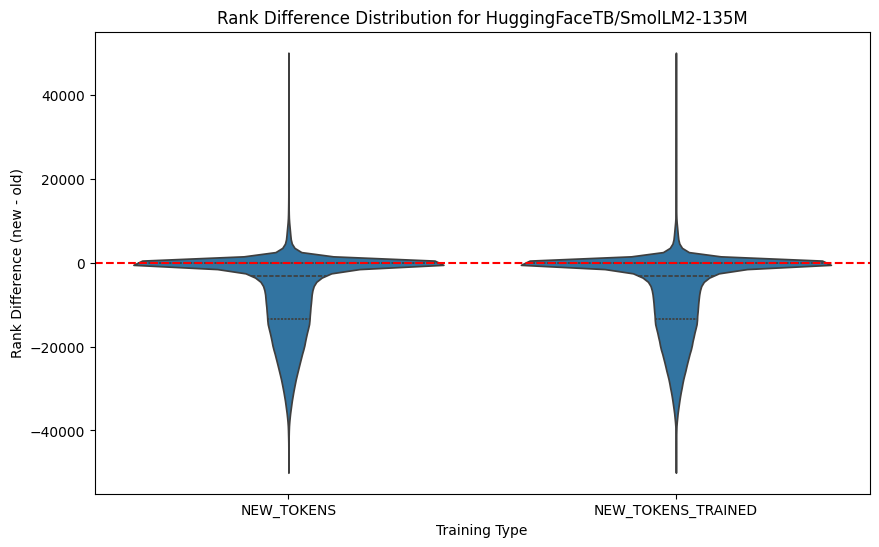
\includegraphics[width=1\textwidth]{Figures//Appendix/violin_smol135M.png}
    \caption{Distribution of rank differences across the entire results data. Negative numbers show preference towards \texttt{new\_token}.}
    \label{fig:violin_rank_dist:smol135M}
\end{figure}
% ---------------------------------------------


% ---------------------------------------------
\subsection*{Model \textit{Qwen/Qwen2.5-1.5B-Instruct}}
\begin{figure}[H]
    \centering
    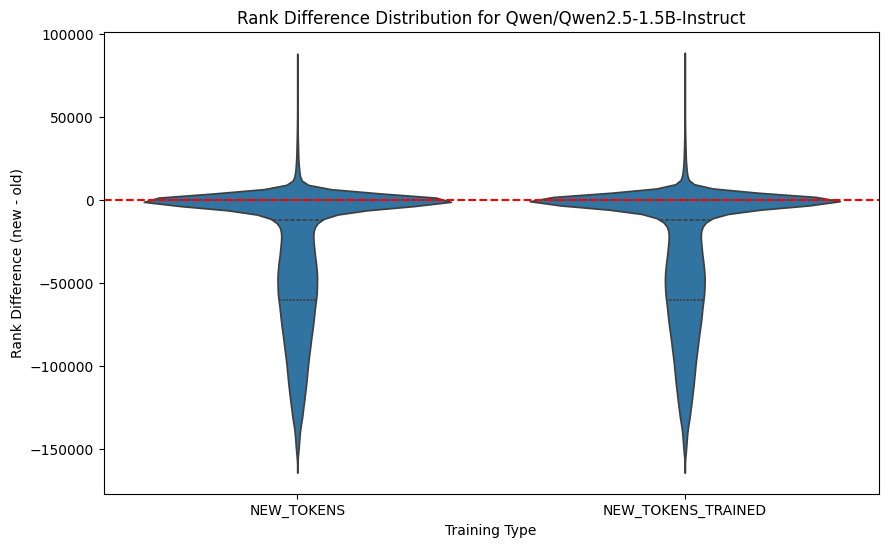
\includegraphics[width=1\textwidth]{Figures//Appendix/violin_qwen.png}
    \caption{Distribution of rank differences across the entire results data. Negative numbers show preference towards \texttt{new\_token}.}
    \label{fig:violin_rank_dist:qwen1.5B}
\end{figure}
% ---------------------------------------------


% ---------------------------------------------
\subsection*{Model \textit{HuggingFaceTB/SmolLM3-3B}}
\begin{figure}[H]
    \centering
    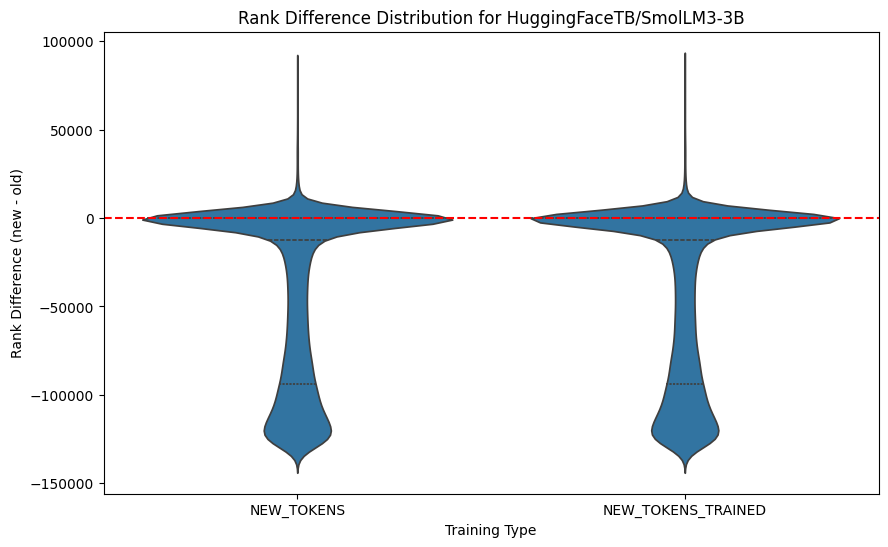
\includegraphics[width=1\textwidth]{Figures//Appendix/violin_smol3B.png}
    \caption{Distribution of rank differences across the entire results data. Negative numbers show preference towards \texttt{new\_token}.}
    \label{fig:violin_rank_dist:smol3B}
\end{figure}
% ---------------------------------------------